\documentclass[11pt,a4paper]{article}
\usepackage[margin=2.3cm]{geometry}
\usepackage{mathptmx}
\usepackage{amsmath}
\usepackage{graphicx}
\usepackage{booktabs}
\usepackage{threeparttable}
\usepackage{makecell}
\usepackage{float}
\usepackage[font=small,labelfont=bf]{caption}
\usepackage{enumitem}
\usepackage{xcolor}
\usepackage{microtype}
\usepackage[colorlinks=true,linkcolor=blue!50!black,citecolor=blue!50!black,urlcolor=blue!50!black]{hyperref}
\usepackage[capitalise,noabbrev]{cleveref}
\graphicspath{{figs/}}
\setlist[itemize,enumerate]{nosep,leftmargin=*}
\setlist[description]{nosep,leftmargin=3em,labelindent=0pt}
\newcommand{\auroc}{AUROC}
\newcommand{\sensninety}{sens@spec90}

\title{\textbf{Twelve to One: Lead-Robust Deep Learning for Multi-label ECG Diagnosis and Wearable Triage on PTB-XL}}
\author{[Author names, Matric No.]\\[2pt] \small BS6204 Deep Learning for Biomedical Science, Nanyang Technological University}
\date{October 2026}

\begin{document}
\maketitle

\begin{abstract}
\noindent Smartwatches record a single-lead electrocardiogram (ECG), but most diagnostic deep-learning models assume the 12-lead clinical ECG. We asked how much multi-label diagnostic ability survives when the input is reduced from 12 leads to wearable-like lead sets, and which diagnoses a reduced lead set could screen for. On PTB-XL (21,388 records, official patient-level folds) we trained baselines, three architectures with different inductive biases (ResNet1d, CNN-BiLSTM, ECG-ViT) and four training strategies (from scratch, supervised transfer, a lead-agnostic ResNet with lead masks, and self-supervised masked signal modelling) on six lead configurations, for five-class diagnosis and normal-versus-abnormal triage (102 training runs, three seeds). Reduced configurations were judged with a pre-specified criterion combining non-inferior AUROC (paired-bootstrap lower bound $\geq -0.02$) and sensitivity $\geq 0.80$ at 90\% specificity. All deep models reached 12-lead macro AUROC 0.915--0.925. Moving to lead I lowered macro AUROC by 0.090 (95\% CI 0.081--0.100), with myocardial infarction losing most ($\Delta$AUROC $-0.128$). No diagnosis met the criterion with lead I; ST/T change with the six chest leads was the only robust exception. Transfer learning and more labels did not close the gap, indicating an information bottleneck; one lead-agnostic model served all six configurations at a cost of 0.003--0.010 AUROC, and self-supervised pre-training improved a 10\%-label Transformer by 0.015 on lead I. Frozen triage models kept their discrimination on 34,815 external records from another hospital, but decision thresholds needed local calibration.
\end{abstract}

\section{Introduction}
\label{sec:intro}

Cardiovascular diseases are the leading cause of death worldwide, accounting for an estimated 19.8 million deaths in 2022, about 32\% of all deaths~\cite{who_cvd}. The 12-lead ECG is the first-line test for many of them: myocardial infarction (MI), ischaemic ST/T changes, conduction disturbances and hypertrophy all leave characteristic traces in the twelve projections of the heart's electrical activity. Deep neural networks now read 12-lead ECGs at a level comparable to cardiologists for many diagnostic statements~\cite{ribeiro2020automatic,strodthoff2021benchmark}, and single-lead networks detect rhythm disorders in ambulatory recordings~\cite{hannun2019cardiologist}.

At the same time, ECG acquisition is moving out of the clinic. Consumer smartwatches record a single limb lead between the wrist and the opposite fingertip, and large studies have shown that wearables can flag atrial fibrillation in the general population~\cite{perez2019apple}. Rhythm, however, is the easy case: it can be read from the timing of beats in any lead. Most structural and ischaemic diagnoses depend on the spatial information that the full 12-lead system provides, and it is unclear how much of it a single lead retains. This matters in practice. If a wearable could reliably screen for some diagnoses, it could decide who needs a full 12-lead ECG; if it cannot, an apparently high average accuracy could give false reassurance.

Published comparisons usually report one averaged metric per lead configuration. An averaged AUROC hides two questions that matter for screening: \emph{which} diagnoses survive lead reduction, and whether the surviving performance is good enough at a clinically useful operating point. We therefore framed lead reduction as a replaceability question with a criterion defined before any reduced-lead result was seen, and applied it to every diagnosis and lead configuration. We addressed three research questions:

\begin{description}
  \item[RQ1] Which architecture and baseline perform best on the 12-lead ECG, and how large is the gap to traditional methods?
  \item[RQ2] How much diagnostic performance is lost as leads are removed, down to a smartwatch-like lead I, and which diagnoses can a reduced lead set still screen for? Can training strategies recover the loss?
  \item[RQ3] How do reduced-lead models behave for normal-versus-abnormal triage, under noise, with fewer labels, with self-supervised pre-training, and on data from another hospital?
\end{description}

Our contributions are:
\begin{enumerate}
  \item A \textbf{pre-specified replaceability criterion} (non-inferior AUROC plus sensitivity at 90\% specificity), applied per diagnosis and per lead configuration, which yields a conclusion matrix rather than a single averaged score (\cref{fig:conclusion}).
  \item \textbf{LA-ResNet}, a lead-agnostic model trained with lead masks that serves all six lead configurations with one set of weights, together with a quantification of its cost relative to dedicated models.
  \item A \textbf{complete wearable evidence chain} under one protocol: diagnosis, triage, noise robustness, label efficiency including self-supervised pre-training, and external validation on 34,815 records from a different hospital.
\end{enumerate}

\section{Related Work}
\label{sec:related}

\paragraph{Deep learning on the 12-lead ECG.} PTB-XL~\cite{wagner2020ptbxl}, released through PhysioNet~\cite{goldberger2000physionet}, made a large, cardiologist-annotated 12-lead dataset with fixed patient-level folds publicly available. Strodthoff et al.~\cite{strodthoff2021benchmark} benchmarked convolutional, recurrent and feature-based models on it; for the five diagnostic superclasses, the best deep models reached macro AUROC between 0.921 and 0.930, and a wavelet-feature network 0.874. ResNet-style one-dimensional convolutional networks~\cite{he2016resnet} performed consistently well, and recurrent models were competitive. Ribeiro et al.~\cite{ribeiro2020automatic} trained a residual network on more than two million 12-lead ECGs and reported performance comparable to or better than that of cardiology residents for six abnormalities. We use the PTB-XL superclass task and folds so that our 12-lead results can be compared with this benchmark.

\paragraph{Reduced-lead and single-lead ECG analysis.} Hannun et al.~\cite{hannun2019cardiologist} showed that a deep network can classify twelve rhythm classes from single-lead ambulatory ECGs. The PhysioNet/Computing in Cardiology Challenge 2021, ``Will Two Do?''~\cite{reyna2021willtwodo}, asked explicitly how reduced lead sets (twelve, six, four, three and two leads) compare for multi-label diagnosis across several databases, including PTB-XL and the Chapman-Shaoxing/Ningbo data~\cite{zheng2020chapman}. Closest to our single-lead question, Davarmanesh et al.~\cite{davarmanesh2024leadI} detected MI from lead I of PTB-XL and reported a test AUC of 0.92 for MI versus normal records. These studies report how well reduced leads classify; they do not ask, with a pre-specified criterion, whether a reduced lead set is good enough to \emph{replace} the 12-lead ECG for each diagnosis, which is our focus.

\paragraph{Transfer and self-supervised learning.} Transfer of representations from a data-rich setting to a data-poor one is standard in deep learning; for ECGs, Mehari and Strodthoff~\cite{mehari2022ssl} showed that self-supervised pre-training on 12-lead data improves downstream PTB-XL performance and robustness. Masked modelling, introduced for language in BERT~\cite{devlin2019bert} and for images in masked autoencoders~\cite{he2022mae}, is a natural pretext task for Transformers~\cite{vaswani2017attention,dosovitskiy2021vit}. We test whether a simple masked-signal pre-training of an ECG Vision Transformer helps when only 10\% of the labels are available, and whether supervised transfer from 12 leads helps reduced-lead models.

\paragraph{Calibration, statistics and interpretability.} Modern networks are often miscalibrated, and temperature scaling fitted on a validation set is a simple remedy~\cite{guo2017calibration}. We report calibration alongside discrimination, use bootstrap confidence intervals~\cite{efron1993bootstrap} with Holm correction for multiple comparisons~\cite{holm1979}, and use Grad-CAM~\cite{selvaraju2017gradcam} and attention maps only as illustrative, not causal, explanations.

\section{Data and Task Definitions}
\label{sec:data}

\subsection{PTB-XL}
We used PTB-XL v1.0.3~\cite{wagner2020ptbxl}, a public collection of 21,799 ten-second, 12-lead resting ECGs from 18,869 patients, annotated by cardiologists with SCP-ECG statements. Following the reference implementation of Strodthoff et al.~\cite{strodthoff2021benchmark}, every diagnostic statement was mapped to one of five diagnostic superclasses---normal ECG (NORM), myocardial infarction (MI), ST/T change (STTC), conduction disturbance (CD) and hypertrophy (HYP)---regardless of its likelihood value; the 21,388 records with at least one superclass were kept. We used the 100\,Hz version (1,000 samples per lead), as in the PTB-XL benchmark; it keeps the waveform content needed for superclass diagnosis while keeping the full experiment grid of more than 100 training runs within the budget of one laptop GPU.

We used the official stratified folds without modification: folds 1--8 for training (17,084 records), fold 9 for validation (2,146) and fold 10 for testing (2,158). The folds keep all records of a patient in one fold, so there is no patient-level leakage. Label prevalence is almost identical across splits (\cref{tab:data}). Signals were z-scored per lead with a mean and standard deviation estimated on the training fold only, and the same transform was applied to validation, test and external data.

\subsection{Tasks}
\textbf{T1 -- multi-label diagnosis.} Five sigmoid outputs, one per superclass; a record may carry several labels.

\noindent\textbf{T2 -- normal-versus-abnormal triage.} One sigmoid output; a record is \emph{abnormal} if it carries any of MI, STTC, CD or HYP. T2 is the simpler question a wearable is most likely to be asked: does this person need a 12-lead ECG? T2 is not the complement of NORM: 51 test records are labelled NORM together with an abnormal superclass, and they count as abnormal in T2. For T1 models we also report a \emph{derived} triage score, $1-P(\text{NORM})$, evaluated against the same T2 label.

\subsection{Lead configurations}
Each model was trained and tested on one of six lead configurations chosen to span clinical and wearable devices (\cref{tab:leads}).

\begin{table}[H]
\centering
\small
\caption{Lead configurations.}
\label{tab:leads}
\begin{tabular}{lll}
\toprule
Configuration & Leads & Rationale \\
\midrule
12lead & all 12 & clinical reference \\
limb6 & I, II, III, aVR, aVL, aVF & limb-only devices, six-lead patches \\
chest6 & V1--V6 & precordial information without limb leads \\
2lead (I + II) & I, II & two-electrode devices \\
leadII & II & classic rhythm strip \\
leadI & I & smartwatch-like single lead \\
\bottomrule
\end{tabular}
\end{table}

\subsection{External cohort}
For external validation (E7) we used the Chapman-Shaoxing/Ningbo database~\cite{zheng2022physionet,zheng2020chapman} (45,152 ten-second 12-lead ECGs at 500\,Hz from two Chinese hospitals), whose diagnoses are SNOMED-CT codes. We mapped codes to the PTB-XL superclasses with a fixed table (``v2 mapping'') that follows the official equivalence list of the PhysioNet/CinC Challenge 2021~\cite{reyna2021willtwodo}; for example, complete right bundle branch block is treated as right bundle branch block. A record was \emph{normal} only if all its codes were sinus-rhythm codes (sinus rhythm, sinus bradycardia, sinus tachycardia, sinus arrhythmia), and \emph{abnormal} if at least one code mapped to MI, STTC, CD or HYP. Records with only unmapped findings (for example atrial fibrillation alone, axis deviation or ectopic beats) were excluded, because PTB-XL's diagnostic superclasses do not cover them. Signals were converted to millivolts, resampled to 100\,Hz with an anti-aliasing polyphase filter, cropped or zero-padded to 10\,s, and records with a flat or non-finite lead were excluded. Of 45,152 records, 34,815 were included (16,092 abnormal, 18,723 normal); 8,971 were excluded for unmapped diagnoses and 1,366 for signal problems (\cref{tab:data}). Two alternative mappings were analysed as sensitivity analyses (\cref{sec:res_triage}).

\begin{table}[H]
\centering
\small
\caption{Cohorts. PTB-XL label prevalence is multi-label (rows do not sum to 100\%). Chapman fractions use all scanned records.}
\label{tab:data}
\begin{tabular}{lrrrrrr}
\toprule
PTB-XL split & Records & NORM & MI & STTC & CD & HYP \\
\midrule
Train (folds 1--8) & 17,084 & 44.5\% & 25.6\% & 24.5\% & 22.9\% & 12.4\% \\
Validation (fold 9) & 2,146 & 44.5\% & 25.2\% & 24.6\% & 23.1\% & 12.5\% \\
Test (fold 10) & 2,158 & 44.6\% & 25.5\% & 24.1\% & 23.0\% & 12.1\% \\
\midrule
\multicolumn{7}{l}{\textbf{Chapman-Shaoxing/Ningbo (external, v2 mapping)}} \\
\multicolumn{5}{l}{Scanned} & \multicolumn{2}{r}{45,152 (100\%)} \\
\multicolumn{5}{l}{Excluded: no mappable diagnosis} & \multicolumn{2}{r}{8,971 (19.9\%)} \\
\multicolumn{5}{l}{Excluded: flat lead / non-finite signal / unreadable header} & \multicolumn{2}{r}{1,290 / 75 / 1} \\
\multicolumn{5}{l}{Included (abnormal / normal)} & \multicolumn{2}{r}{34,815 (16,092 / 18,723)} \\
\bottomrule
\end{tabular}
\end{table}

\section{Methods}
\label{sec:methods}

All models were written from scratch in PyTorch and trained with one shared training loop, so that differences between models come from the architecture or strategy and not from the training recipe (\cref{fig:design}).

\begin{figure}[t]
\centering
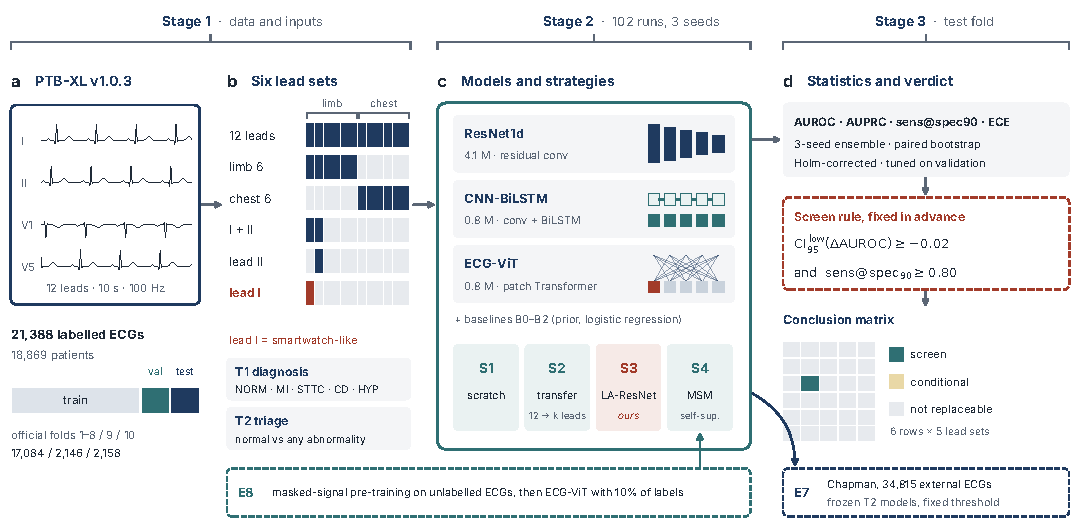
\includegraphics[width=\linewidth]{figA_study_design.pdf}
\caption{Study design. \textbf{a}, PTB-XL records and the official patient-level folds. \textbf{b}, six lead configurations, from 12 leads to the smartwatch-like lead I, each trained and tested separately, for diagnosis (T1) and triage (T2). \textbf{c}, three architectures with different inductive biases and four training strategies (S3 is our lead-agnostic model), plus baselines B0--B2; 102 runs with three seeds. \textbf{d}, test-fold statistics, the screen rule fixed before any result, and the resulting conclusion matrix. Dashed boxes: self-supervised pre-training with 10\% labels (E8) and external validation of frozen models on 34,815 Chapman ECGs (E7), which reports external metrics only.}
\label{fig:design}
\end{figure}

\subsection{Baselines}
\begin{itemize}
  \item \textbf{B0 (prior)} predicts each class's training prevalence for every record (AUROC $=0.5$ by construction).
  \item \textbf{B1 (pre-specified)} is a logistic regression ($C=0.1$) on the standardised signal after $4\times$ average pooling (3,000 features for 12 leads).
  \item \textbf{B2 (feature baseline).} B1 performed at chance (\cref{sec:res_arch}) because a fixed time sample means different things in different records: beats are not aligned across recordings. B2 therefore summarises each lead with 22 shift-invariant features (13 amplitude statistics, 2 slope statistics, relative power in 5 frequency bands, and the dominant autocorrelation period and its strength as a rhythm estimate) and fits the same logistic regression. B2 was added after B1 failed; B1 is kept and reported unchanged.
\end{itemize}

\subsection{Architectures: three inductive biases}
\begin{itemize}
  \item \textbf{ResNet1d} (4.07\,M parameters) is a one-dimensional residual network~\cite{he2016resnet}: a stride-2 convolution (kernel 15) and max-pooling stem, eight basic residual blocks (kernel 7) widening from 64 to 256 channels in three stride-2 stages, concatenated global average and max pooling, dropout 0.2 and a linear head. Its receptive field is 1,291 samples, longer than the 10\,s input. \emph{Bias:} local, translation-equivariant morphology detectors stacked hierarchically.
  \item \textbf{CNN-BiLSTM} (0.79\,M) combines a convolutional stem that down-samples by 4 (250 time steps), a two-layer bidirectional LSTM~\cite{hochreiter1997lstm} (hidden size 128, dropout 0.3) and additive attention pooling over time. \emph{Bias:} local feature extraction followed by sequential modelling of beat-to-beat context.
  \item \textbf{ECG-ViT} (0.82\,M) is a one-dimensional Vision Transformer~\cite{dosovitskiy2021vit}. The recording is split into 50 non-overlapping 200\,ms patches (20 samples $\times$ all leads), linearly embedded ($D=128$), prefixed with a learnable CLS token and summed with a sinusoidal position encoding, then passed through four pre-LayerNorm Transformer blocks~\cite{vaswani2017attention} (four heads, MLP width 512) with hand-written multi-head self-attention; the CLS token feeds the classifier. \emph{Bias:} weak locality prior, global interactions between all patches from the first layer.
\end{itemize}

\subsection{Training strategies}
\begin{itemize}
  \item \textbf{S1 -- from scratch:} one model per lead configuration.
  \item \textbf{S2 -- supervised transfer} starts from the 12-lead ResNet1d of the same seed. The first convolution is replaced by one with the reduced number of input leads, and the 12-lead filters of the leads that remain are copied into it. \emph{Fine-tune:} all layers are trained, the new input layer and head at the base learning rate and the backbone at $0.1\times$ (discriminative learning rate). \emph{Frozen:} only the new input layer and the head are trained (lead I only).
  \item \textbf{S3 -- LA-ResNet (lead-agnostic; our design)} is one ResNet1d with 24 input channels: the 12 standardised leads, with missing leads set to zero, plus 12 constant 0/1 mask channels that tell the network which leads are real. During training each record is shown with all 12 leads (probability 0.5), one of the five reduced configurations (0.3) or a random lead subset (0.2). Early stopping uses the mean validation AUROC over all six configurations, so a single checkpoint serves every configuration at test time.
  \item \textbf{S4 -- self-supervised pre-training (E8).} ECG-ViT is first trained without labels by masked signal modelling, following the masked-modelling idea of BERT and masked autoencoders~\cite{devlin2019bert,he2022mae}: 8 of the 50 patches ($\approx$15\%) are replaced by a learnable mask embedding and the network reconstructs their standardised samples (mean squared error on the hidden patches only). Pre-training used all training-fold records without labels (one encoder for 12lead and one for leadI; up to 100 epochs; early stopping on the validation reconstruction error). The encoder was then fine-tuned with a new classification head on 10\% of the training patients' labels, with all layers at the same learning rate as S1.
\end{itemize}

\subsection{Shared training recipe}
All supervised models used binary cross-entropy with logits, AdamW~\cite{loshchilov2019adamw} (learning rate $10^{-3}$, weight decay $10^{-2}$), a one-cycle learning-rate schedule~\cite{smith2019onecycle} with 10\% warm-up, batch size 128, gradient-norm clipping at 1.0 and mixed precision on the GPU. Training ran for at most 50 epochs with early stopping on validation macro AUROC (patience 10); the best weights were kept as a deep copy and restored. Training-time augmentation consisted of per-lead amplitude scaling ($\sigma=0.1$), a baseline offset ($\sigma=0.05$), additive Gaussian noise ($\sigma=0.02$) and a random circular shift of up to $\pm0.5$\,s. No hyper-parameter was tuned for any individual model. Every configuration in the main grid was trained with three seeds (0, 1, 2), except the ablations and label-efficiency runs, which used seed 0 as pre-specified.

\subsection{Experiments}
\Cref{tab:experiments} lists the experiment grid: 102 supervised runs in the main grid and 14 runs in E8. Subsets of training patients in E5 and E8 were drawn per seed at the patient level, and both arms of E8 used the same subset within a seed.

\begin{table}[H]
\centering
\small
\caption{Experiment grid.}
\label{tab:experiments}
\begin{tabular}{lp{7.2cm}p{5.2cm}}
\toprule
ID & Question & Runs \\
\midrule
E0 & Baselines B0--B2 (12lead, leadI; T1, T2) & CPU only \\
E1 & Architectures on 12 leads & 3 models $\times$ 3 seeds = 9 \\
E1b & Ablations: no residual; kernel 3/15/31; vanilla RNN; class-weighted loss & 6 (seed 0) \\
E2 & Reduced leads, trained from scratch & 3 models $\times$ 5 configurations $\times$ 3 seeds = 45 \\
E3 & Training strategies & S2 fine-tune 15 + S2 frozen 3 + S3 3 = 21 \\
E4 & T2 triage & ResNet1d $\times$ \{12lead, leadI\} $\times$ 3 + LA-ResNet $\times$ 3 = 9 \\
E5 & Label efficiency (10/25/50\% of training patients) & 12 (seed 0) \\
E7 & External validation (frozen models) & 0 \\
E8 & Self-supervised pre-training & 2 pre-training + 12 fine-tuning \\
\bottomrule
\end{tabular}
\end{table}

\section{Evaluation Protocol}
\label{sec:eval}

\paragraph{Metrics.} The primary metric is macro AUROC on the test fold, because it is threshold-free and comparable across classes with different prevalence. Because AUROC alone can hide poor performance at clinically useful operating points, we also report AUPRC; sensitivity at 90\% specificity (\sensninety, the operating point of the success criterion); F1, PPV and NPV at per-class thresholds tuned on the validation fold; the Brier score; and the expected calibration error (ECE, 15 bins) before and after temperature scaling fitted on the validation fold~\cite{guo2017calibration}.

\paragraph{Pre-specified success criterion.} Before any reduced-lead result was seen, we defined when a reduced configuration can \emph{screen} for a diagnosis in place of the 12-lead reference:
\begin{enumerate}
  \item \emph{non-inferior discrimination}: the lower bound of the paired-bootstrap 95\% confidence interval of $\Delta$AUROC (reduced $-$ 12-lead) is at least $-0.02$; and
  \item \emph{useful operating point}: \sensninety\ $\geq 0.80$.
\end{enumerate}
A cell meeting both conditions is \emph{screen}, one of the two \emph{conditional}, and neither \emph{not replaceable}. The reference is the 12-lead model of the same architecture family trained from scratch (ResNet1d for LA-ResNet and S2). The margin was varied to 0.01 and 0.03 as a sensitivity analysis. The \emph{primary approach} shown in the conclusion matrix was chosen on the validation fold only: among approaches covering all five reduced configurations, the one with the highest mean validation macro AUROC.

\paragraph{Uncertainty and statistical tests.} Predicted probabilities of the three seeds were averaged (seed ensemble) before computing conclusion-matrix and paired-test statistics; across-seed mean $\pm$ SD is reported for single models. Confidence intervals come from 1,000 record-level bootstrap resamples of the test fold~\cite{efron1993bootstrap}. Paired comparisons use the same resamples for both models and a two-sided bootstrap $p$-value; with 1,000 resamples, $p<0.001$ is the resolution limit. The 29 paired comparisons of architectures, lead sets and strategies were adjusted together with the Holm method~\cite{holm1979}, and we use ``significant'' only for Holm-adjusted $p<0.05$.

\paragraph{Robustness, subgroups and interpretability.} At test time we added white Gaussian noise to the raw signal at signal-to-noise ratios of 20, 10, 5 and 0\,dB. We report AUROC by sex and age group ($<$50, 50--70, $>$70 years) as descriptive estimates, seed and heterogeneous ensembles, and an inter-model disagreement analysis. Grad-CAM~\cite{selvaraju2017gradcam} was computed for ResNet1d and LA-ResNet and, for ECG-ViT, on the input of the last Transformer block, together with its attention matrix.

\paragraph{Leakage control and reproducibility.} Splits follow the official patient-level folds. The standardiser, decision thresholds, temperature, early stopping and the choice of primary approach use the training or validation folds only; nothing was tuned on the test fold or the external cohort. All runs are reproducible from the released scripts, and a CPU regression test on synthetic data had to give a bit-identical result before and after every code change.

\section{Results}
\label{sec:results}

\subsection{Baselines and architectures on 12 leads}
\label{sec:res_arch}
All three deep models reached a test macro AUROC between 0.915 and 0.925 (\cref{tab:main}), within the range reported for the PTB-XL superclass benchmark (0.921--0.930)~\cite{strodthoff2021benchmark}. Seed ensembles reached 0.930, 0.929 and 0.922. ResNet1d and CNN-BiLSTM did not differ (ensemble difference $+0.0005$ [$-0.0020$, $+0.0031$], Holm-adjusted $p=1.000$), whereas both outperformed ECG-ViT (ResNet1d $-$ ECG-ViT $+0.0077$ [$+0.0043$, $+0.0108$]; CNN-BiLSTM $-$ ECG-ViT $+0.0071$ [$+0.0038$, $+0.0106$]; both Holm-adjusted $p<0.001$).

The pre-specified raw-waveform logistic regression B1 performed at chance (macro AUROC 0.512; NORM AUROC 0.70 on the training fold but 0.52 on validation), confirming that a linear model on unaligned time samples does not generalise. The shift-invariant feature baseline B2 reached 0.863, close to the feature-based wavelet network of the PTB-XL benchmark (0.874)~\cite{strodthoff2021benchmark}, but remained well below the deep models.

\begin{table}[t]
\centering
\small
\caption{Test-fold results on 12 leads (T1). Deep models: mean $\pm$ SD over three seeds; seed-ensemble AUROC with bootstrap 95\% CI. Baselines are single deterministic fits.}
\label{tab:main}
\setlength{\tabcolsep}{4pt}
\resizebox{\linewidth}{!}{%
\begin{tabular}{lccccc}
\toprule
Model & Macro AUROC & Macro AUPRC & \sensninety & ECE & Ensemble AUROC [95\% CI] \\
\midrule
B0 prior & 0.500 & 0.259 & 0.000 & 0.002 & -- \\
B1 raw-signal LR & 0.512 & 0.286 & 0.142 & 0.111 & -- \\
B2 feature LR & 0.863 & 0.700 & 0.627 & 0.028 & -- \\
\midrule
ResNet1d & 0.9227 $\pm$ 0.0015 & 0.816 $\pm$ 0.004 & 0.777 $\pm$ 0.010 & 0.033 $\pm$ 0.001 & 0.9298 [0.9231, 0.9367] \\
CNN-BiLSTM & \textbf{0.9253} $\pm$ 0.0013 & \textbf{0.817} $\pm$ 0.003 & 0.773 $\pm$ 0.003 & 0.039 $\pm$ 0.006 & 0.9292 [0.9225, 0.9363] \\
ECG-ViT & 0.9147 $\pm$ 0.0009 & 0.795 $\pm$ 0.001 & 0.752 $\pm$ 0.007 & 0.043 $\pm$ 0.005 & 0.9221 [0.9152, 0.9295] \\
\bottomrule
\end{tabular}}
\end{table}

The single-seed ablations changed AUROC by at most 0.012 relative to the seed-0 ResNet1d (0.9211; \cref{app:ablation}). Because these differences are of the order of the across-seed spread and were measured with one seed, we do not interpret them as evidence that one variant is better.

\subsection{How much is lost when leads are removed}
Performance fell as leads were removed, with a clear step between two-lead and single-lead inputs (\cref{fig:ladder}). For ResNet1d, the seed-ensemble macro AUROC dropped by 0.031 with limb6, 0.024 with chest6, 0.033 with leads I + II, 0.071 with lead II and 0.090 with lead I (0.930 $\rightarrow$ 0.840; 95\% CI of the drop 0.081--0.100; all Holm-adjusted $p<0.001$). The three architectures followed the same pattern; with lead I they reached 0.835 (ResNet1d), 0.838 (CNN-BiLSTM) and 0.824 (ECG-ViT).

The loss was not uniform across diagnoses (\cref{fig:perclass}). With lead I, MI suffered most (ResNet1d 0.918 $\rightarrow$ 0.787), followed by CD (0.914 $\rightarrow$ 0.821) and HYP (0.902 $\rightarrow$ 0.807), whereas STTC (0.934 $\rightarrow$ 0.874) and NORM (0.946 $\rightarrow$ 0.885) were better preserved. The six chest leads kept almost all STTC information (0.926 versus 0.934 with 12 leads) but lost more for MI (0.864) than the six limb leads (0.882).

\begin{figure}[t]
\centering
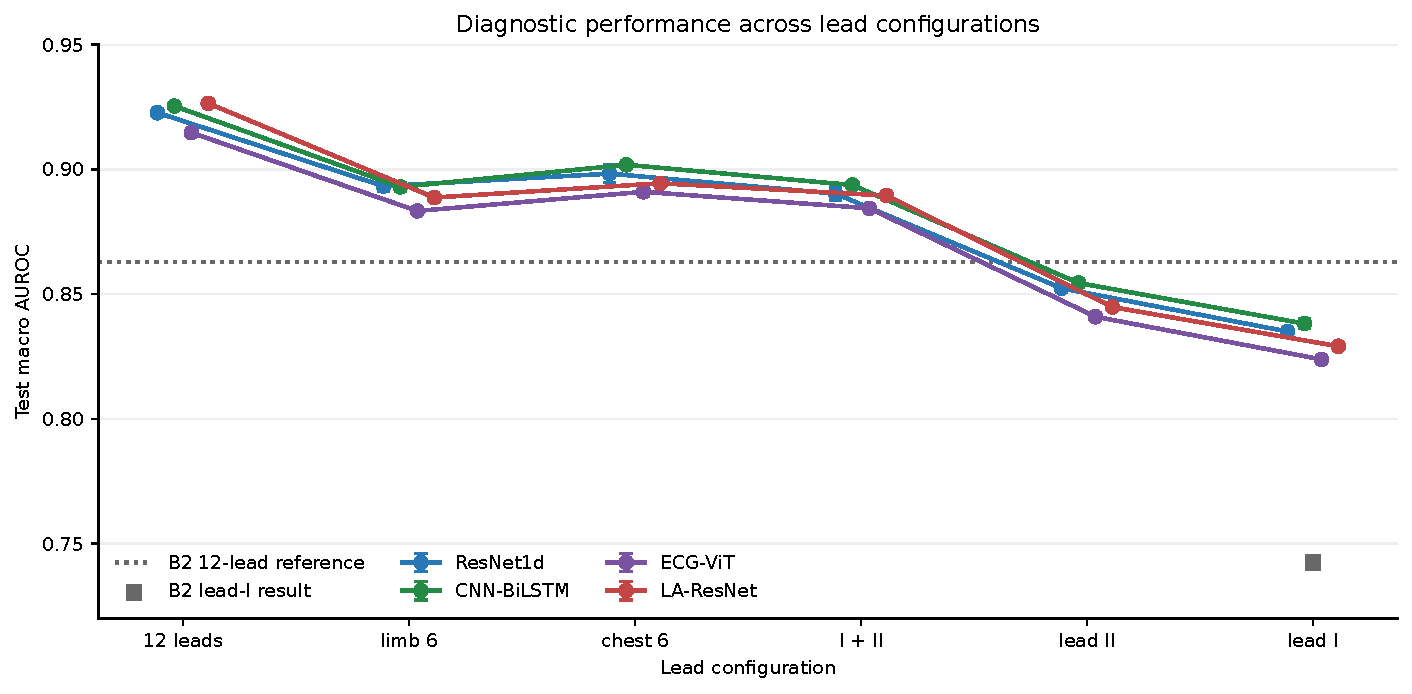
\includegraphics[width=0.92\linewidth]{figB_lead_ladder.pdf}
\caption{Test macro AUROC (mean $\pm$ SD over three seeds) across lead configurations for the three architectures trained from scratch and the single LA-ResNet model. The dotted line is the B2 feature baseline on 12 leads; the square is B2 on lead I.}
\label{fig:ladder}
\end{figure}

\begin{figure}[t]
\centering
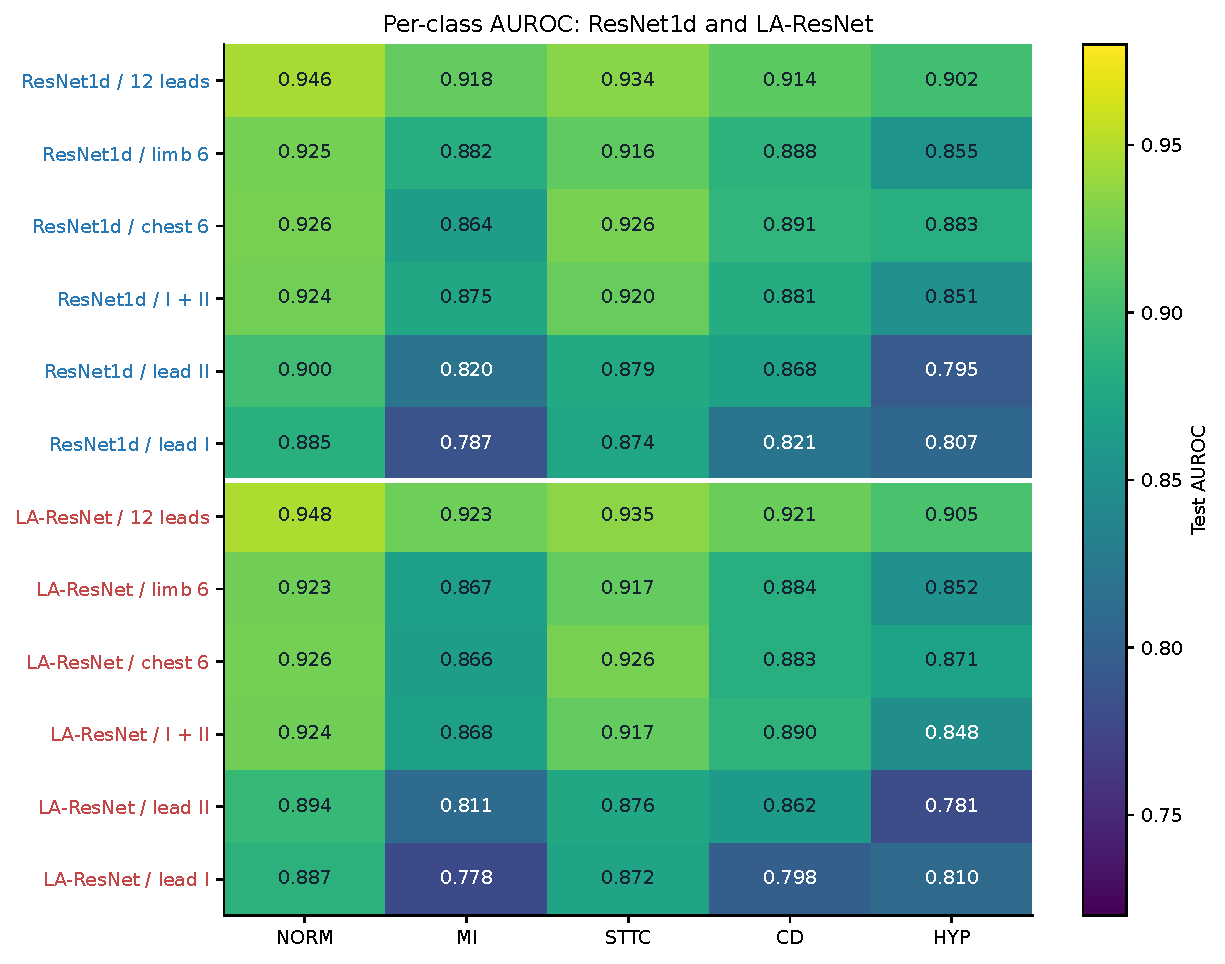
\includegraphics[width=0.72\linewidth]{figC_per_class_heatmap.pdf}
\caption{Per-class test AUROC (mean over three seeds) for dedicated ResNet1d models and the single LA-ResNet model across lead configurations.}
\label{fig:perclass}
\end{figure}

\subsection{Can a reduced lead set replace the 12-lead ECG?}
\label{sec:res_conclusion}
\Cref{fig:conclusion} applies the pre-specified criterion to every diagnosis and reduced configuration for the primary approach, CNN-BiLSTM, which was selected on the validation fold (its mean validation AUROC over the reduced configurations, 0.8866, was 0.0001 above that of ResNet1d). Of 30 cells (five diagnoses plus derived triage, times five configurations), 29 were \emph{not replaceable} and one met the \emph{screen} criterion: STTC with the six chest leads ($\Delta$AUROC $-0.004$ [$-0.010$, $+0.001$], \sensninety\ 0.84). This result did not depend on the choice of approach: STTC with chest6 was \emph{screen} for all five evaluated approaches ($\Delta$AUROC $-0.0045$ to $-0.0089$; lower CI bounds $-0.0097$ to $-0.0155$; \sensninety\ 0.82--0.84).

No diagnosis could be screened with lead I. The largest gap was MI ($\Delta$AUROC $-0.128$ [$-0.147$, $-0.107$], \sensninety\ 0.45), and even the derived triage score reached only 0.71 sensitivity at 90\% specificity. The verdicts were unchanged with a margin of 0.01. With a margin of 0.03, 8 of the 29 cells became \emph{conditional} (non-inferior AUROC but \sensninety\ $<0.80$) and none became \emph{screen}. The operating-point requirement is demanding: even the 12-lead CNN-BiLSTM reached a mean \sensninety\ of only about 0.74 for MI and 0.71 for HYP, so these classes could not have met the second condition with any input.

\begin{figure}[t]
\centering
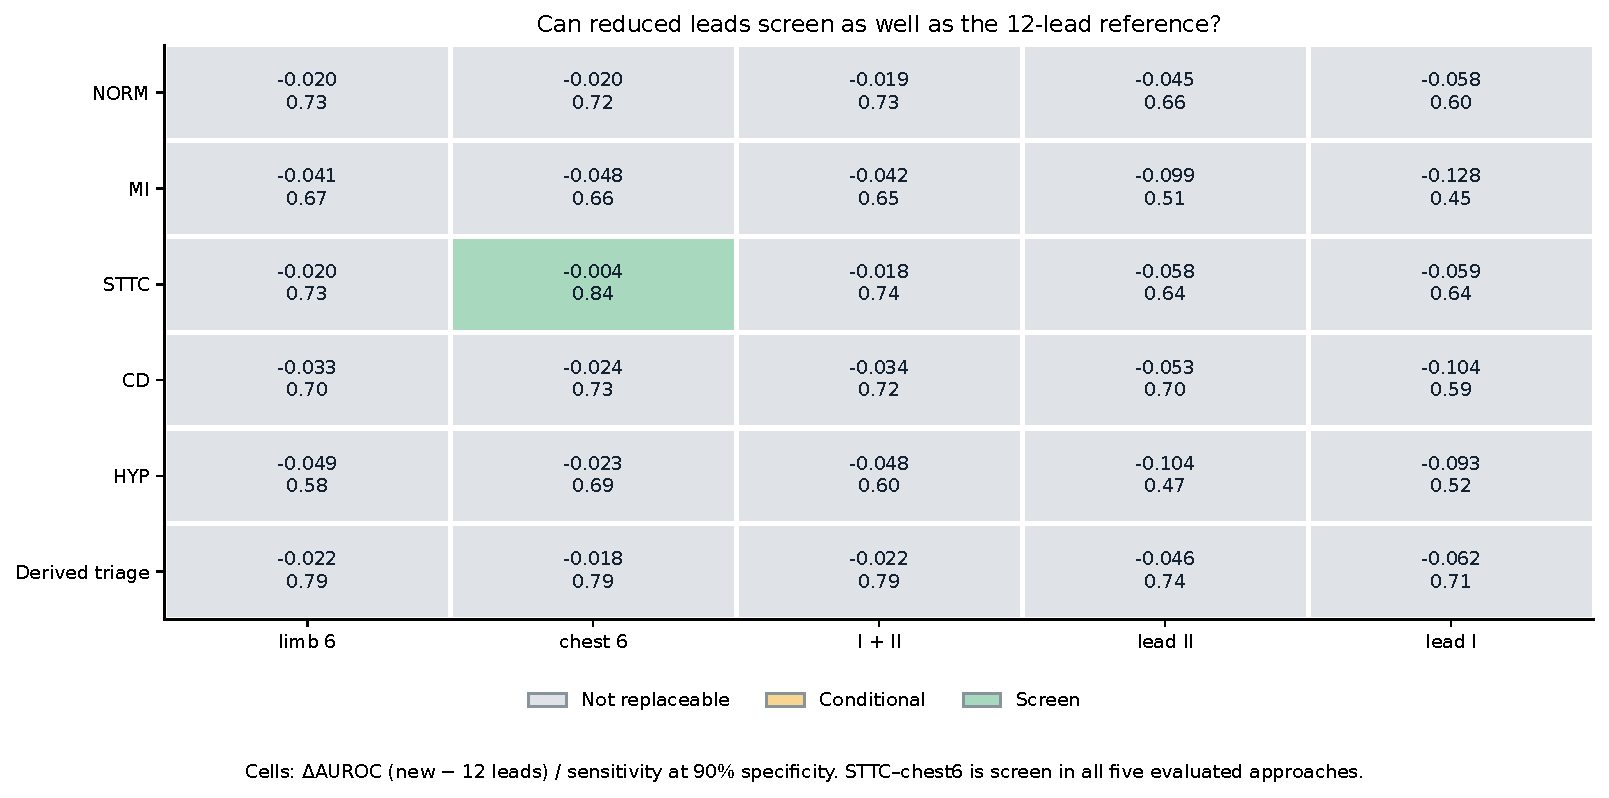
\includegraphics[width=\linewidth]{figD_conclusion_matrix.pdf}
\caption{Conclusion matrix for the validation-selected primary approach (CNN-BiLSTM). Each cell gives $\Delta$AUROC versus the 12-lead reference and the sensitivity at 90\% specificity; the colour gives the pre-specified verdict. STTC with the six chest leads is the only \emph{screen} cell and is \emph{screen} for all five evaluated approaches.}
\label{fig:conclusion}
\end{figure}

\subsection{Do training strategies recover the loss?}
Neither strategy recovered the information lost with the leads (\cref{tab:strategies}, \cref{fig:ladder}). Supervised transfer from the 12-lead ResNet1d changed the seed-ensemble AUROC by between $-0.0023$ and $+0.0022$ across the five configurations, with no comparison significant after Holm correction; freezing the backbone was worse than training from scratch with lead I ($-0.0078$ [$-0.0117$, $-0.0037$]).

A single LA-ResNet checkpoint served all six configurations. With 12 leads its mean AUROC (0.9264 $\pm$ 0.0004) was at least as high as that of the dedicated ResNet1d (0.9227 $\pm$ 0.0015). On reduced configurations it was 0.0033--0.0095 below the five dedicated scratch models, significantly so for chest6, lead II and lead I. The lead-agnostic design thus trades a small, measurable loss for the convenience of one model that accepts any of the six lead sets.

\begin{table}[t]
\centering
\small
\begin{threeparttable}
\caption{Training strategies versus dedicated ResNet1d trained from scratch: paired seed-ensemble $\Delta$AUROC (T1).}
\label{tab:strategies}
\begin{tabular}{llccc}
\toprule
Configuration & Strategy & $\Delta$AUROC & 95\% CI & Holm $p$ \\
\midrule
limb6 & S2 fine-tune & $-0.0003$ & [$-0.0031$, $+0.0025$] & 1.000 \\
 & S3 LA-ResNet & $-0.0044$ & [$-0.0079$, $-0.0011$] & 0.064 \\
chest6 & S2 fine-tune & $+0.0022$ & [$-0.0007$, $+0.0050$] & 0.732 \\
 & S3 LA-ResNet & $-0.0054$ & [$-0.0092$, $-0.0018$] & 0.018 \\
2lead & S2 fine-tune & $+0.0011$ & [$-0.0017$, $+0.0041$] & 1.000 \\
 & S3 LA-ResNet & $-0.0033$ & [$-0.0070$, $+0.0002$] & 0.462 \\
leadII & S2 fine-tune & $-0.0017$ & [$-0.0052$, $+0.0018$] & 1.000 \\
 & S3 LA-ResNet & $-0.0095$ & [$-0.0148$, $-0.0045$] & $<$0.001 \\
leadI & S2 fine-tune & $-0.0023$ & [$-0.0052$, $+0.0006$] & 0.732 \\
 & S2 frozen & $-0.0078$ & [$-0.0117$, $-0.0037$] & $<$0.001 \\
 & S3 LA-ResNet & $-0.0080$ & [$-0.0124$, $-0.0034$] & $<$0.001 \\
\bottomrule
\end{tabular}
\begin{tablenotes}\footnotesize
\item Holm adjustment covers all 29 paired comparisons (architectures, lead sets, strategies). $p<0.001$ is the resolution of 1,000 bootstrap resamples.
\end{tablenotes}
\end{threeparttable}
\end{table}

\subsection{Robustness, label efficiency and self-supervised pre-training}
\paragraph{Noise.} With 12 leads, all architectures degraded gracefully down to 5\,dB (\cref{fig:noise}). With lead I, severe noise changed the ranking: at 0\,dB the three-seed mean AUROC was 0.759 for ResNet1d but 0.686 for CNN-BiLSTM, although CNN-BiLSTM had been slightly better on clean signals (0.838 versus 0.835). This is a descriptive comparison under synthetic white noise.

\paragraph{Label efficiency.} With 12 leads, training on 10\% of the patients (1,681 records) cost 0.040 AUROC relative to the full training set (ResNet1d seed 0: 0.881 versus 0.921). With lead I, the same reduction cost only 0.023 (0.812 versus 0.835), and even the 10\%-data 12-lead model (0.881) outperformed the full-data lead-I model by 0.047 (\cref{fig:labels}). The single-lead gap is therefore limited mainly by the information in the input rather than by the amount of training data.

\paragraph{Self-supervised pre-training (E8).} Masked signal modelling improved ECG-ViT trained on 10\% of the labels (\cref{tab:ssl}): the seed-ensemble AUROC rose by $+0.0065$ [$+0.0020$, $+0.0112$] with 12 leads and by $+0.0149$ [$+0.0091$, $+0.0210$] with lead I (both significant after Holm correction for the two comparisons), and the across-seed SD fell from 0.0078 to 0.0006 (12 leads) and from 0.0026 to 0.0005 (lead I). Both pre-training runs reached the 100-epoch limit (best epochs 98 and 96), so convergence was not established and the gain is best read as a lower bound. Pre-training narrowed, but did not reverse, ECG-ViT's low-label disadvantage: its 10\%-label mean AUROC (0.876 with 12 leads, 0.810 with lead I) was comparable to, not better than, ResNet1d trained from scratch on 10\% of the labels (seed 0: 0.881 and 0.812).

\begin{figure}[t]
\centering
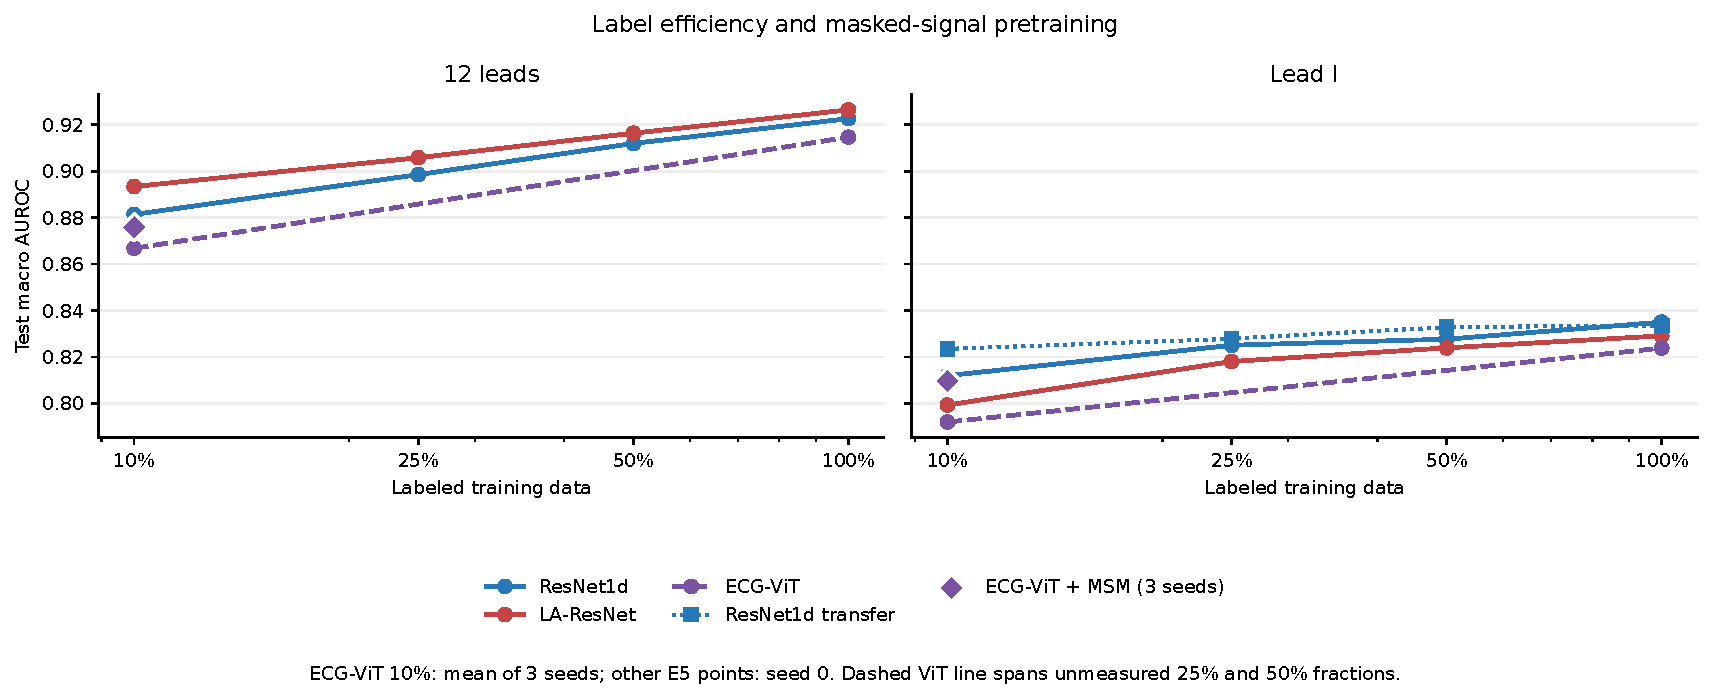
\includegraphics[width=\linewidth]{figE_label_efficiency.pdf}
\caption{Label efficiency with 12 leads and lead I. Points are seed 0 except ECG-ViT at 10\% (mean of three seeds); diamonds show ECG-ViT with masked-signal pre-training. Dashed lines span unmeasured fractions.}
\label{fig:labels}
\end{figure}

\begin{table}[t]
\centering
\small
\caption{Masked-signal pre-training (MSM) versus training from scratch for ECG-ViT with 10\% of the labels: three-seed mean $\pm$ SD and seed-ensemble AUROC [95\% CI]; paired difference on seed-ensemble predictions. The full-data ECG-ViT is a reference only.}
\label{tab:ssl}
\begin{tabular}{lcccc}
\toprule
Leads & Scratch & MSM & MSM $-$ scratch [95\% CI] & Full-data ViT \\
\midrule
12lead & \makecell{0.8668 $\pm$ 0.0078\\0.8860 [0.8771, 0.8955]} & \makecell{0.8759 $\pm$ 0.0006\\0.8924 [0.8837, 0.9012]} & \makecell{$+0.0065$ [$+0.0020$, $+0.0112$]\\$p=0.006$} & 0.9221 \\
\addlinespace
leadI & \makecell{0.7919 $\pm$ 0.0026\\0.8053 [0.7938, 0.8185]} & \makecell{0.8096 $\pm$ 0.0005\\0.8203 [0.8087, 0.8318]} & \makecell{$+0.0149$ [$+0.0091$, $+0.0210$]\\$p<0.001$} & 0.8287 \\
\bottomrule
\end{tabular}
\end{table}

\begin{figure}[t]
\centering
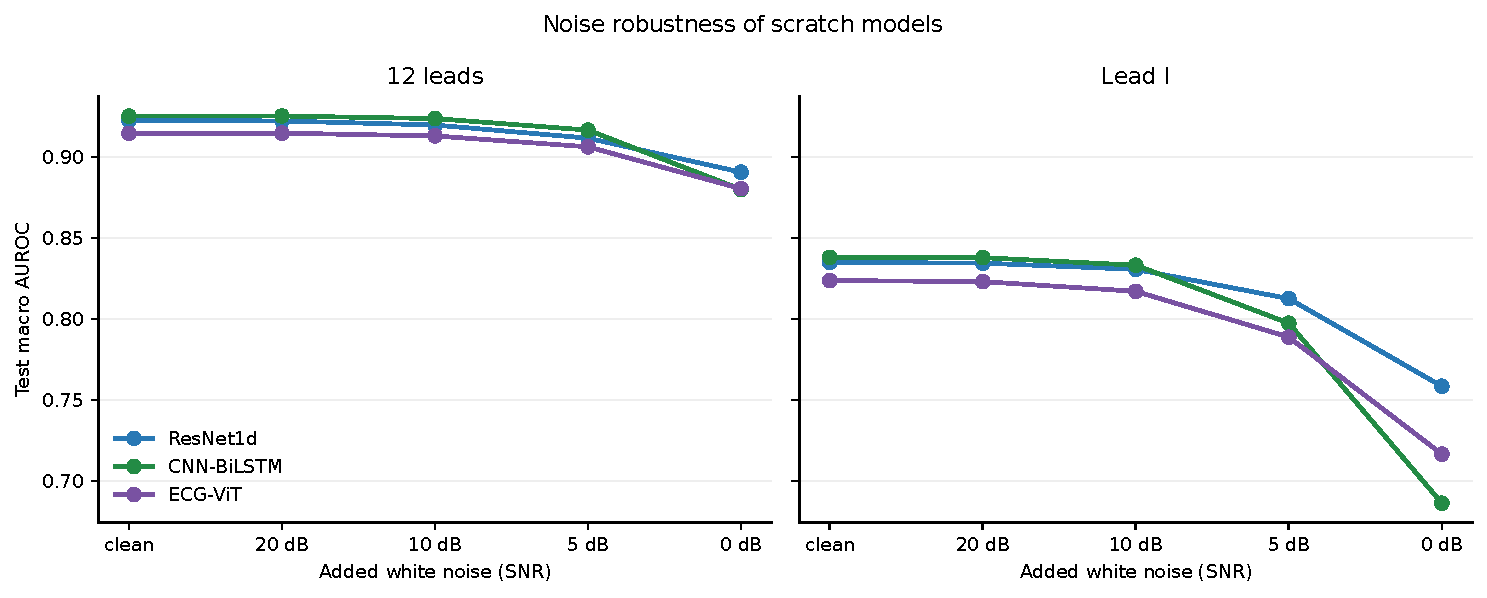
\includegraphics[width=0.7\linewidth]{figG_noise_robustness.pdf}
\caption{Test macro AUROC under additive white noise at test time, for 12 leads and lead I (three-seed means).}
\label{fig:noise}
\end{figure}

\subsection{Triage on PTB-XL and in an external hospital}
\label{sec:res_triage}
\paragraph{Internal triage.} Dedicated T2 models reached a seed-ensemble AUROC of 0.940 with 12 leads and 0.878 with lead I (ResNet1d); sensitivity at 90\% specificity fell from 0.83 to 0.71 (\cref{fig:triage}). A dedicated T2 model gave no apparent advantage over the derived score $1-P(\text{NORM})$ of T1 models (lead I: 0.705--0.708 versus 0.700--0.711). All reduced configurations were \emph{not replaceable} for triage; even the best, chest6 with LA-ResNet, narrowly missed both conditions ($\Delta$AUROC $-0.021$ [$-0.027$, $-0.015$], \sensninety\ 0.79).

\paragraph{External validation (E7).} Applied without retraining or re-tuning to 34,815 Chapman records, the frozen T2 models kept their discrimination (\cref{tab:external}, \cref{fig:triage}): ResNet1d reached 0.955 [0.953, 0.957] with 12 leads and 0.916 [0.913, 0.919] with lead I, compared with 0.940 and 0.878 on the PTB-XL test fold; LA-ResNet gave 0.957 and 0.912. The values depended on the label definition. Under the archived first mapping (v1) they were 0.953 and 0.910; when ``left ventricular high voltage''---a voltage criterion rather than a diagnosis of hypertrophy---was also counted as abnormal (v2 + LVHV), they fell to 0.936 and 0.880, close to the internal values. Across the three mappings, external AUROC ranged from 0.936 to 0.957 with 12 leads and from 0.875 to 0.916 with lead I.

Thresholds chosen on the PTB-XL validation fold for 90\% specificity transferred approximately but not exactly: on the external cohort they gave a sensitivity/specificity of 0.905/0.864 with 12 leads and 0.797/0.903 with lead I (ResNet1d). Because the external target is restricted (strictly sinus-rhythm negatives, mapped diagnoses only) and the case mix differs, the higher external AUROC should not be read as better generalisation, and it does not change the lead-I verdicts of \cref{sec:res_conclusion}, which are defined on PTB-XL.

\begin{figure}[t]
\centering
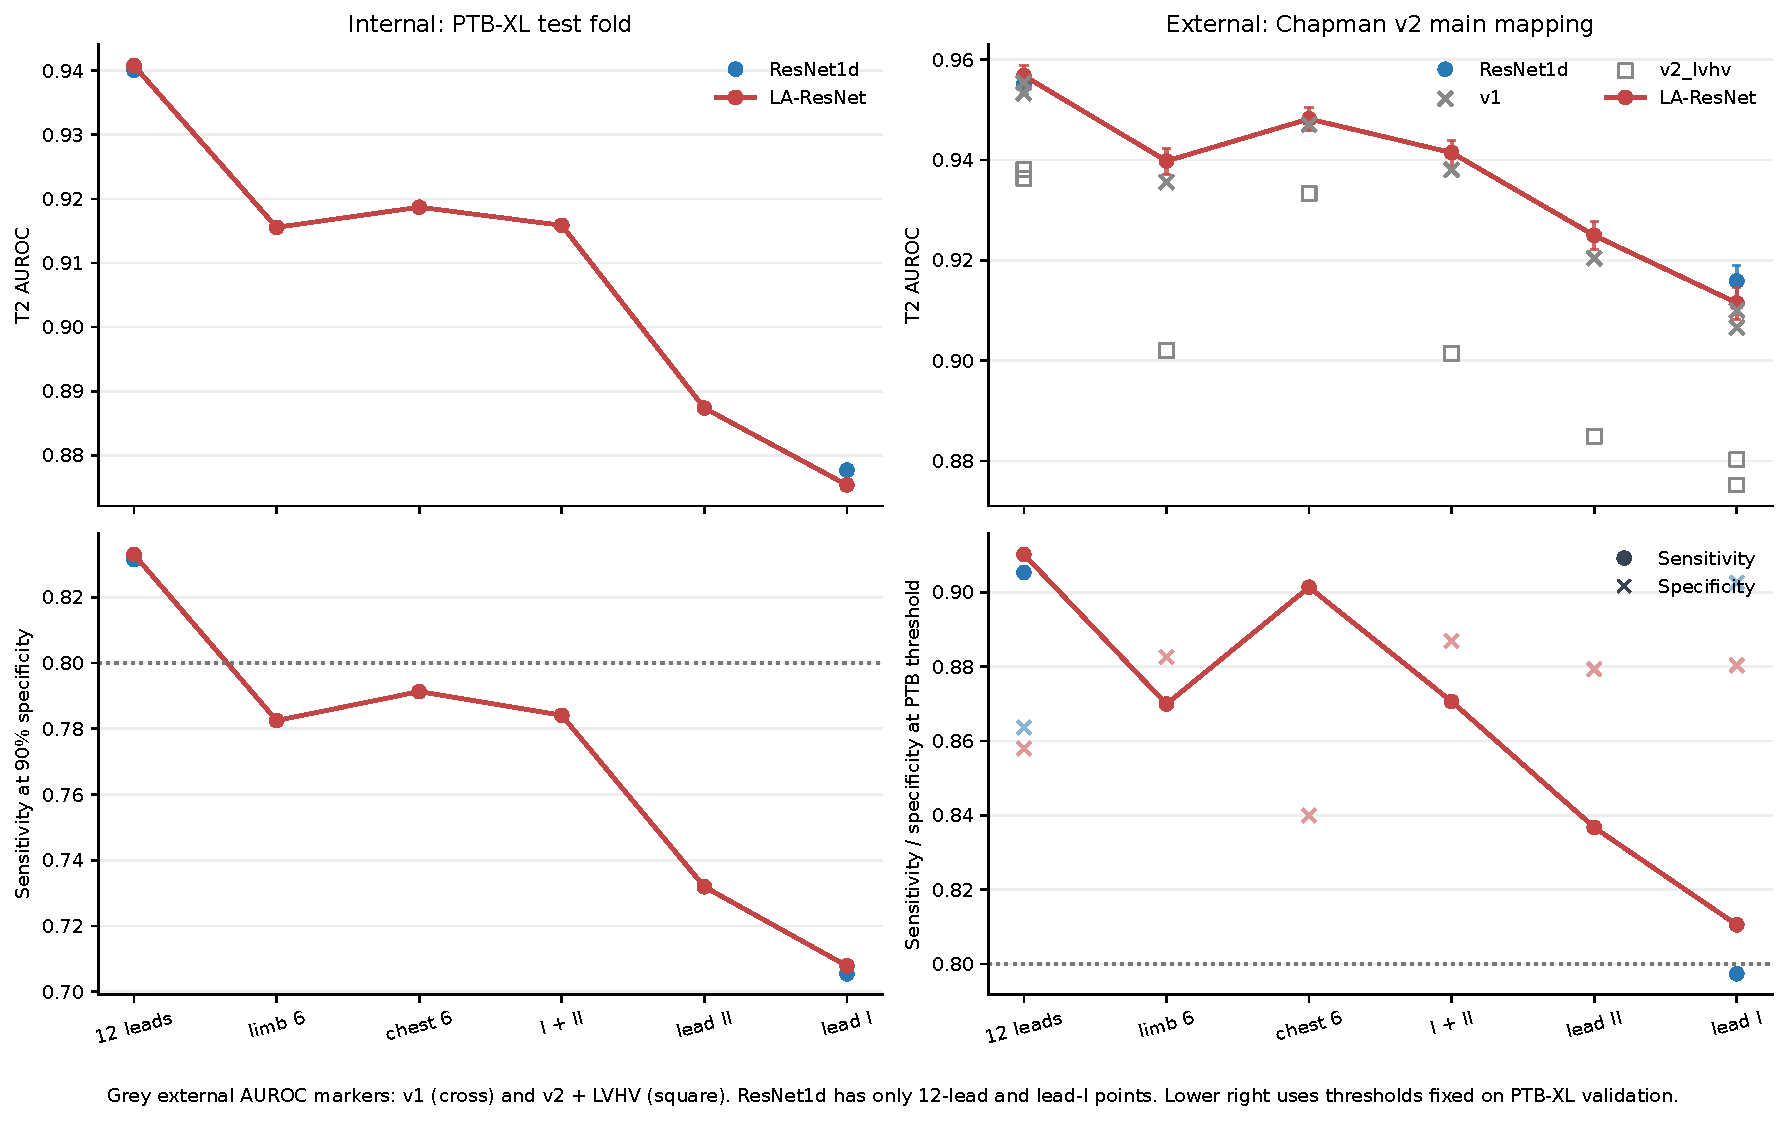
\includegraphics[width=\linewidth]{figF_triage_external.pdf}
\caption{Triage (T2). Left: PTB-XL test fold. Right: Chapman external cohort under the v2 mapping, with v1 and v2 + LVHV as sensitivity analyses (grey markers). Lower right: sensitivity and specificity at thresholds fixed on the PTB-XL validation fold.}
\label{fig:triage}
\end{figure}

\begin{table}[t]
\centering
\small
\caption{External validation of frozen T2 models on the Chapman cohort under three label mappings (v2 = main analysis). Sens/spec: sensitivity and specificity at the threshold chosen for 90\% specificity on the PTB-XL validation fold. The negative set (strictly sinus-rhythm records) is identical across mappings, so specificity at the transported threshold does not change; LA-ResNet under v1 and v2 + LVHV is listed in the results files.}
\label{tab:external}
\setlength{\tabcolsep}{4pt}
\resizebox{\linewidth}{!}{%
\begin{tabular}{lllcccc}
\toprule
Mapping & Model & Leads & $n$ (pos.) & External AUROC [95\% CI] & Internal AUROC & Sens/spec at PTB thr. \\
\midrule
v2 & ResNet1d & 12lead & 34,815 (16,092) & 0.955 [0.953, 0.957] & 0.940 & 0.905 / 0.864 \\
v2 & ResNet1d & leadI & 34,815 (16,092) & 0.916 [0.913, 0.919] & 0.878 & 0.797 / 0.903 \\
v2 & LA-ResNet & 12lead & 34,815 (16,092) & 0.957 [0.955, 0.959] & 0.941 & 0.910 / 0.858 \\
v2 & LA-ResNet & leadI & 34,815 (16,092) & 0.912 [0.908, 0.915] & 0.875 & 0.811 / 0.880 \\
\midrule
v1 & ResNet1d & 12lead & 31,364 (12,641) & 0.953 [0.951, 0.956] & 0.940 & 0.901 / 0.864 \\
v1 & ResNet1d & leadI & 31,364 (12,641) & 0.910 [0.907, 0.914] & 0.878 & 0.788 / 0.903 \\
v2+LVHV & ResNet1d & 12lead & 37,313 (18,590) & 0.936 [0.934, 0.939] & 0.940 & 0.851 / 0.864 \\
v2+LVHV & ResNet1d & leadI & 37,313 (18,590) & 0.880 [0.877, 0.884] & 0.878 & 0.728 / 0.903 \\
\bottomrule
\end{tabular}}
\end{table}

\subsection{Ensembles, uncertainty, subgroups and interpretability}
Averaging the three seeds improved the macro AUROC in all 38 model--configuration--task combinations (mean gain $+0.0045$). A heterogeneous ensemble of the three architectures reached 0.932 with 12 leads and 0.842 with lead I, only marginally above the best seed ensemble. Inter-model disagreement flagged harder records: among the 20\% of test records on which the models disagreed most, the label error rate was 0.196 versus 0.087 for the remaining records with 12 leads ($2.3\times$) and 0.256 versus 0.141 with lead I ($1.8\times$). Disagreement could therefore be used to refer uncertain recordings for review, although we did not test such a referral policy.

Subgroup AUROCs were broadly similar (for example, lead-I CNN-BiLSTM 0.846 in 1,110 male and 0.835 in 1,048 female records; \cref{app:subgroups}); without subgroup confidence intervals these estimates are descriptive and do not establish a fairness difference.

Grad-CAM maps of ResNet1d were broad and covered most of the recording (\cref{fig:explain}). This is expected: the receptive field of the last block (1,291 samples) exceeds the input length, so the maps indicate coarse regions rather than individual waves. The ECG-ViT attention matrix showed a strong vertical stripe at one key token (around 4.8--5.0\,s), a pattern consistent with an attention sink, to which we do not assign a physiological meaning. These visualisations are illustrative and are not causal clinical explanations.

\begin{figure}[t]
\centering
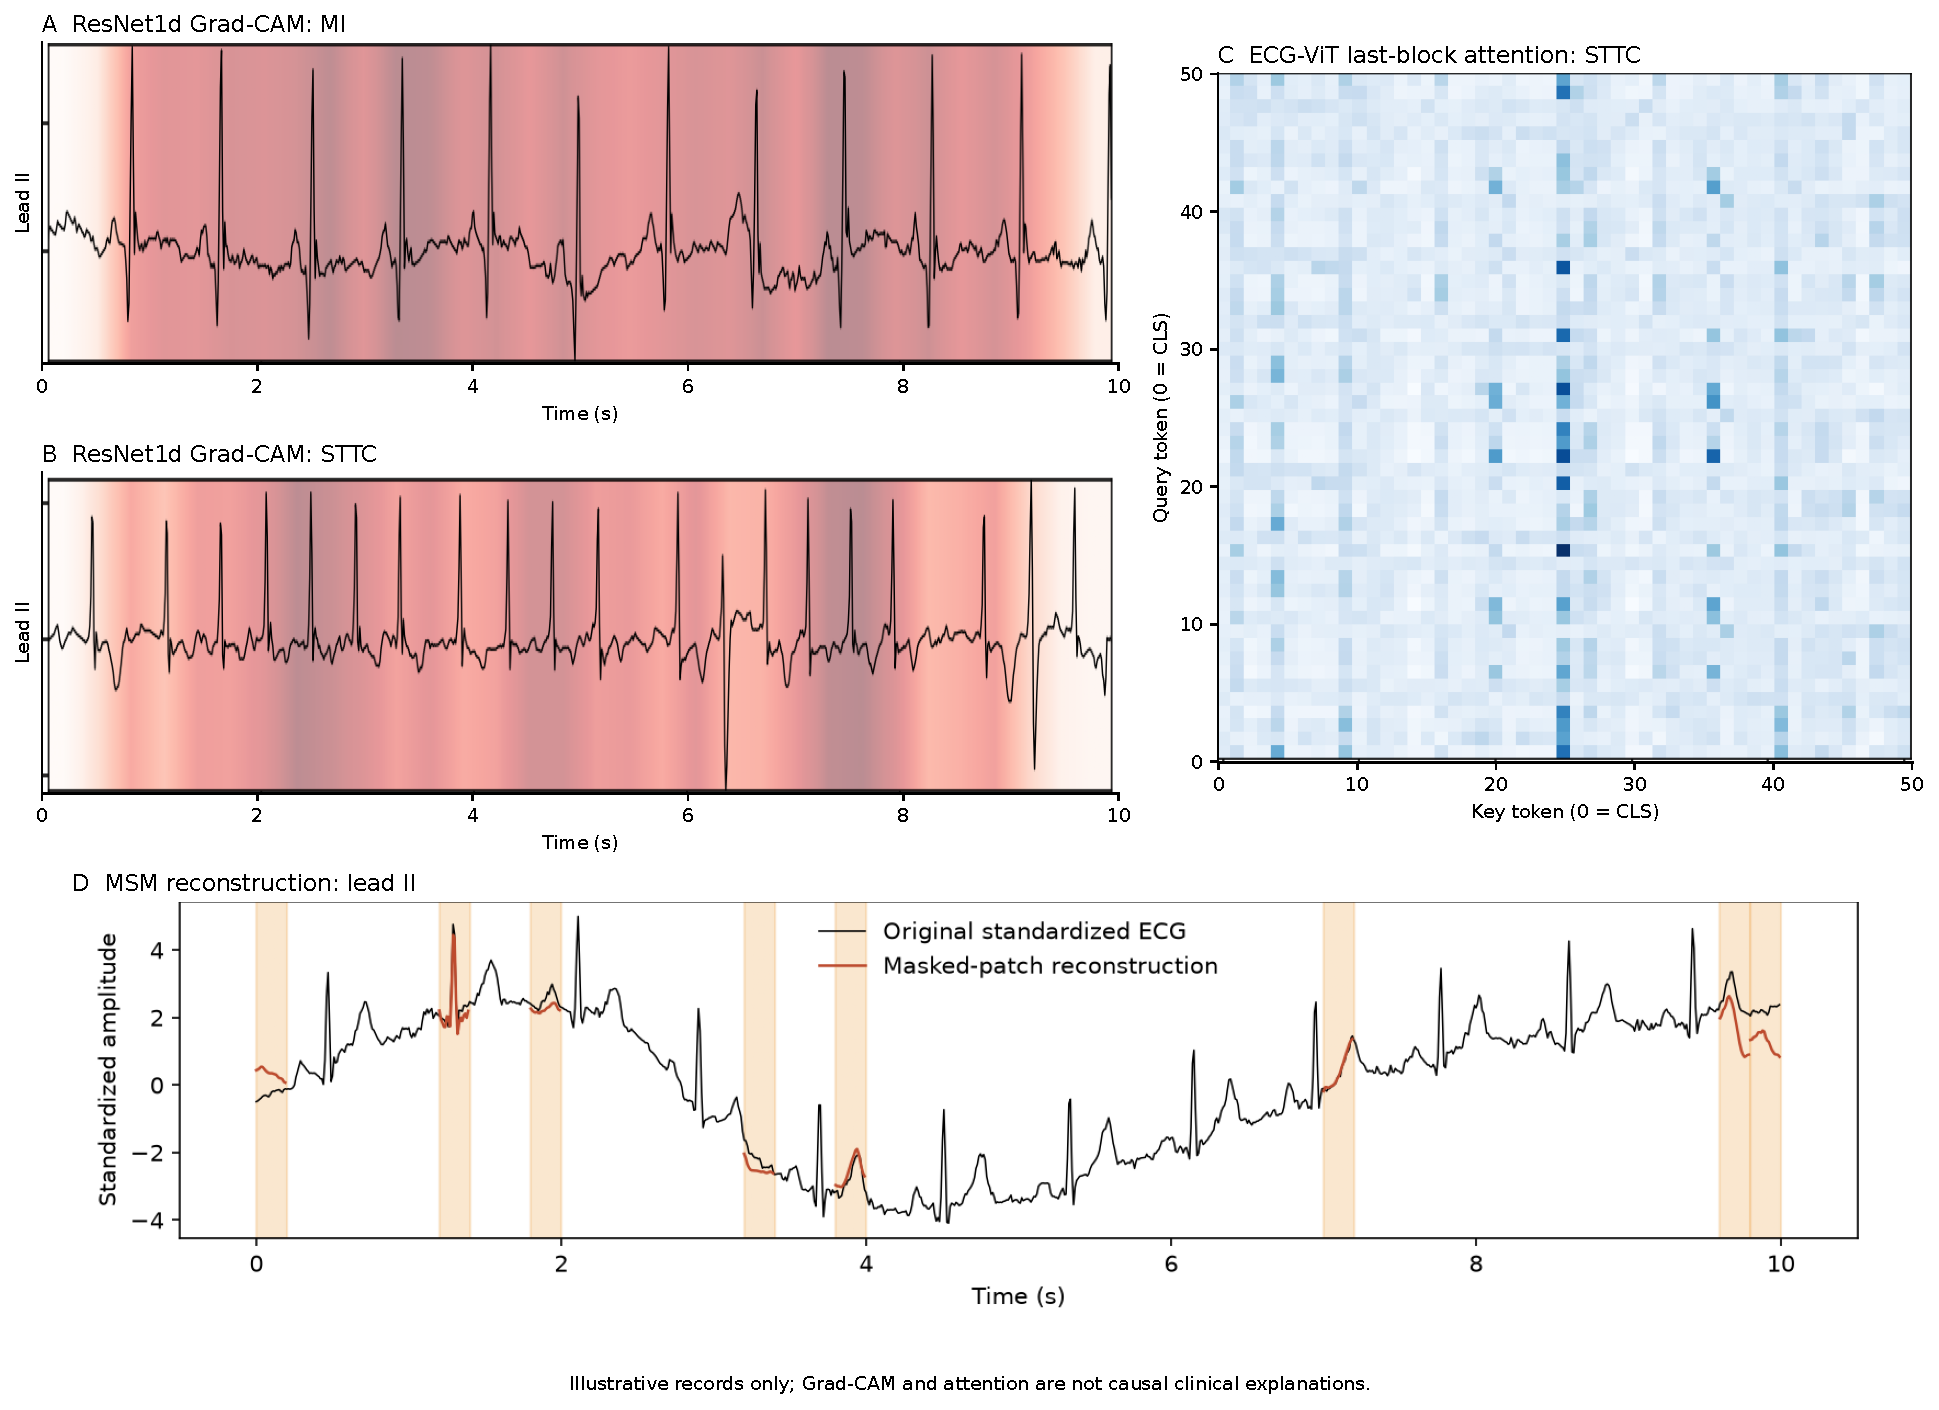
\includegraphics[width=\linewidth]{figH_explainability.pdf}
\caption{Illustrative explanations: ResNet1d Grad-CAM for MI and STTC (lead II), ECG-ViT last-block attention for an STTC record, and a masked-signal reconstruction example (shaded patches were hidden).}
\label{fig:explain}
\end{figure}

\section{Discussion}
\label{sec:discussion}

\paragraph{Twelve to one is too far for diagnosis.} Our central result is negative and, we think, useful: under a criterion fixed in advance, no superclass diagnosis can be screened from lead I, and reduced configurations with two or six leads replace the 12-lead ECG only for ST/T change with the chest leads. The average loss for lead I (0.09 AUROC) is large, but the conclusion matrix shows where it comes from. The pattern is consistent with the spatial coverage of each configuration. Lead I views the heart's electrical axis from the lateral direction only, so inferior changes (seen mainly in II, III and aVF) and anterior or septal changes (seen mainly in V1--V4) are largely invisible to it; MI, which is defined by such regional changes, lost most. Hypertrophy criteria rely heavily on precordial voltages, and HYP was better preserved by the chest leads (0.883) than by the limb leads (0.855). ST/T changes are often most visible in the precordial leads, which is in line with STTC surviving the chest-lead configuration almost unchanged. These anatomical explanations are hypotheses consistent with the per-class results, not something our experiments test directly.

\paragraph{The bottleneck is information, not data or training.} Three independent observations point the same way. Supervised transfer from 12 leads did not improve any reduced-lead model after correction; adding ten times more training data improved the lead-I model by only 0.023 AUROC, whereas a 12-lead model trained on 10\% of the data still beat it; and different architectures converged to similar lead-I performance (0.824--0.838). Better optimisation of single-lead models is therefore unlikely to close the gap; additional information---a second lead, a chest lead or repeated recordings---is needed.

\paragraph{What a wearable can do.} Triage is the more realistic use. With lead I, models still separated normal from abnormal ECGs with AUROC 0.88 on PTB-XL and 0.92 on the external cohort, but their sensitivity at 90\% specificity (0.71 internally) fell short of what we required for a stand-alone screen. Such a model could support, but not replace, the decision to obtain a 12-lead ECG. Two of our findings matter for deployment. First, the lead-agnostic LA-ResNet handled every lead configuration with one set of weights at a cost of 0.003--0.010 AUROC, which is attractive for devices whose available leads vary. Second, inter-model disagreement identified records with roughly twice the error rate, which could be used to refer uncertain recordings for human review.

\paragraph{Operating point and criterion.} The second condition of the criterion (sensitivity $\geq0.80$ at 90\% specificity) is strict: even 12-lead models reached only about 0.74 for MI and 0.71 for HYP. We kept the criterion unchanged after seeing the results; relaxing it would change the verdicts for some cells but not for lead I, where the non-inferiority condition already fails by a wide margin (\cref{fig:conclusion}). The sensitivity analysis on the margin (0.01 and 0.03) did not produce any additional \emph{screen} cell.

\paragraph{Self-supervision and Transformers.} ECG-ViT was the weakest architecture with full labels and gained most from masked-signal pre-training with 10\% labels, consistent with the view that Transformers, which have weak inductive biases, benefit from pre-training. The gain was modest, and our pre-training had not converged within 100 epochs, so a longer or larger pre-training stage may help more. We did not compare masked modelling with other self-supervised objectives such as contrastive learning~\cite{mehari2022ssl}.

\paragraph{External validation.} Frozen models kept their discrimination on records from another country and hospital system, which suggests that what they learned on PTB-XL is not specific to its recording conditions. The higher external AUROC must not be over-interpreted. The external target was restricted by design (only strictly sinus-rhythm negatives and mapped diagnoses), PTB-XL keeps diagnostic statements of any likelihood and thus contains label noise that lowers internal AUROC, and the external positives were dominated by ST/T changes. When borderline voltage-only findings were counted as abnormal, the external AUROC fell to the internal level. Thresholds also shifted, so any deployment would need local recalibration.

\paragraph{Comparison with previous work.} Our 12-lead results (0.915--0.925) lie within the PTB-XL superclass benchmark (0.921--0.930)~\cite{strodthoff2021benchmark}, and our feature baseline (0.863) is close to its wavelet-feature model (0.874). Davarmanesh et al.~\cite{davarmanesh2024leadI} reported an AUC of 0.92 for MI versus normal records from lead I. Our lead-I MI AUROC was 0.80 for the primary approach, but the tasks differ: we classify MI against all other records, including other abnormalities, in a multi-label setting, so the numbers should not be compared directly.

\paragraph{Limitations.}
\begin{itemize}
  \item \emph{Single training source and simulated wearables.} All models were trained on PTB-XL at 100\,Hz. ``Lead I'' is lead I of a clinical recording, not a smartwatch recording, which differs in electrode placement, contact quality, motion artefacts and duration. The noise experiment used synthetic white noise rather than real wearable artefacts.
  \item \emph{Label definitions.} Superclass labels include low-likelihood statements, and the external mapping from SNOMED codes to superclasses is approximate; external results varied with the mapping.
  \item \emph{Statistical scope.} Ablations and label-efficiency curves used one seed; subgroup analyses have no confidence intervals; ECG-ViT pre-training had not converged.
  \item \emph{Fairness of comparison.} All models shared one training recipe without per-model tuning. This makes comparisons fair but means that no model is at its individual best, and the architectures differ in parameter count (0.8--4.1\,M).
  \item \emph{Interpretability.} Grad-CAM and attention maps are coarse and illustrative; they are not validated clinical explanations.
\end{itemize}

\paragraph{Future work.} Natural next steps are to evaluate on genuine smartwatch recordings paired with 12-lead ECGs, to test which \emph{additional} single lead (for example a chest lead obtainable by placing the watch on the chest) recovers most information, to tune the operating point for a two-stage triage pathway, and to extend self-supervised pre-training to larger unlabelled ECG collections.

\section{Conclusion}
\label{sec:conclusion}

\textbf{RQ1.} On 12-lead PTB-XL, ResNet1d and CNN-BiLSTM performed equally well (macro AUROC 0.923 and 0.925) and better than ECG-ViT (0.915); all clearly outperformed a shift-invariant feature baseline (0.863), whereas a linear model on the raw signal failed (0.512).

\textbf{RQ2.} Removing leads cost 0.024--0.033 AUROC for six- and two-lead configurations and 0.090 for lead I, with MI affected most. Under the pre-specified criterion, no diagnosis can be screened from lead I; ST/T change with the six chest leads was the only configuration--diagnosis pair that could replace the 12-lead ECG, consistently across five approaches. Supervised transfer did not recover the loss, while one lead-agnostic model served all six configurations at a small cost.

\textbf{RQ3.} Single-lead triage reached AUROC 0.88 but only 0.71 sensitivity at 90\% specificity, short of a stand-alone screen. Severe noise changed which architecture was best on lead I; more labels helped lead-I models little, pointing to an information bottleneck; masked-signal pre-training improved a 10\%-label Transformer, most on lead I (+0.015). Frozen triage models kept their discrimination on 34,815 records from another hospital, but thresholds needed local calibration.

Twelve to one is too far for diagnosis: a single wearable lead can support triage, but it cannot replace the 12-lead ECG for the five diagnostic superclasses studied here.


\bibliographystyle{ieeetr}
\bibliography{refs}

\clearpage
\appendix
\section{Course concepts used in the implementation}
\label{app:course}

\begin{table}[H]
\centering
\small
\caption{Where course concepts (Lectures 1--8) appear in the code base.}
\begin{tabular}{p{1.4cm}p{6.6cm}p{6.4cm}}
\toprule
Lecture & Concept & Implementation \\
\midrule
L1 & Reproducible seeding; scaler fitted on training data only & \texttt{src/utils.py}; per-lead standardiser in \texttt{src/data.py} \\
L2--L3 & 1-D convolution, stride, padding; layer summaries & ResNet1d and convolutional stems; \texttt{torchinfo} summaries \\
L4 & RNN/LSTM; BCE with logits; class weighting; gradient clipping; early stopping with deep-copied best weights & CNN-BiLSTM and vanilla-RNN ablation; \texttt{run\_epoch}/\texttt{train\_model} in \texttt{src/train.py} \\
L5 & Controlled comparison; majority/prior baseline; receptive field; CNN + recurrent hybrid & E1/E1b design; B0; receptive-field sweep (kernel 3--31); CNN-BiLSTM \\
L6 & Hand-written query/key/value attention; residual + LayerNorm; positional encoding & \texttt{MultiHeadSelfAttention} and pre-LN blocks in \texttt{src/models.py} \\
L7 & Vision Transformer: patches, CLS token, sinusoidal encoding; AdamW; TensorBoard & ECG-ViT; optimiser and logging in \texttt{src/train.py} \\
L8 & ResNet; transfer learning with discriminative learning rates; ensembles; Grad-CAM (including for Transformers) & S2 transfer; seed and heterogeneous ensembles; \texttt{src/gradcam.py} \\
\bottomrule
\end{tabular}
\end{table}

\section{Hyper-parameters}
\label{app:hparams}

\begin{table}[H]
\centering
\small
\caption{Shared training settings (identical for all supervised models).}
\begin{tabular}{ll}
\toprule
Setting & Value \\
\midrule
Input & 100\,Hz, 10\,s (1,000 samples), per-lead z-score from training fold \\
Loss & binary cross-entropy with logits (class weighting only in the E1b ablation) \\
Optimiser & AdamW, learning rate $10^{-3}$, weight decay $10^{-2}$ \\
Schedule & one-cycle, 10\% warm-up \\
Batch size / max epochs & 128 / 50 \\
Early stopping & validation macro AUROC, patience 10, best weights restored \\
Gradient clipping & global norm 1.0 \\
Augmentation & amplitude scale $\sigma=0.1$, offset $\sigma=0.05$, noise $\sigma=0.02$, circular shift $\pm0.5$\,s \\
Transfer (S2) & backbone learning rate $\times0.1$ (fine-tune) or frozen \\
LA-ResNet (S3) & full 12 leads 0.5, reduced configuration 0.3, random subset 0.2 \\
MSM pre-training (S4) & 8/50 patches masked, MSE on masked patches, $\leq$100 epochs, patience 10 \\
Seeds & 0, 1, 2 (ablations and label-efficiency runs: seed 0) \\
Hardware & NVIDIA RTX 3060 Laptop GPU (6\,GB), mixed precision \\
\bottomrule
\end{tabular}
\end{table}

\section{Ablations}
\label{app:ablation}

\begin{table}[H]
\centering
\small
\caption{Single-seed ablations on 12 leads (seed 0, test macro AUROC). Differences of this size are comparable to the across-seed spread and are not interpreted as evidence that one variant is better.}
\begin{tabular}{lc}
\toprule
Variant & Macro AUROC \\
\midrule
ResNet1d (reference, kernel 7) & 0.9211 \\
ResNet1d without residual connections & 0.9166 \\
ResNet1d kernel 3 / 15 / 31 & 0.9233 / 0.9187 / 0.9152 \\
ResNet1d with class-weighted loss & 0.9242 \\
CNN-BiLSTM (LSTM) & 0.9258 \\
CNN-BiLSTM with vanilla RNN & 0.9279 \\
\bottomrule
\end{tabular}
\end{table}

\begin{figure}[H]
\centering
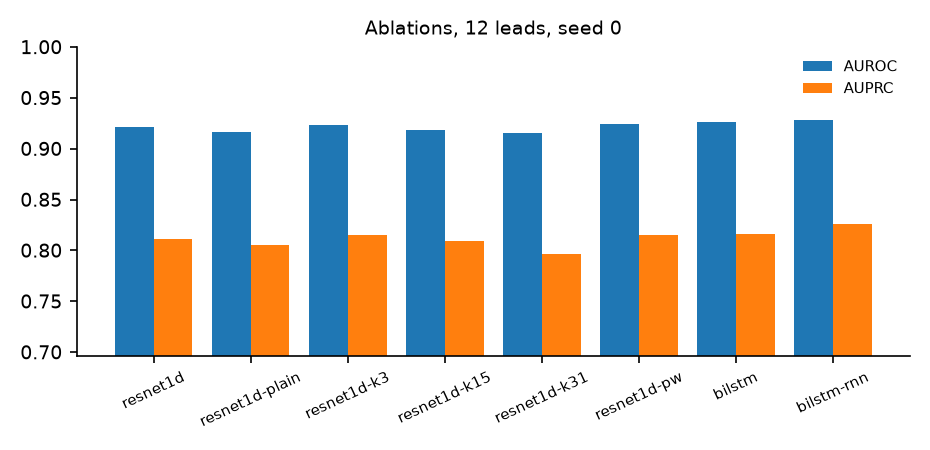
\includegraphics[width=0.7\linewidth]{fig9_ablations.png}
\caption{Ablations on 12 leads (seed 0): macro AUROC and AUPRC.}
\end{figure}

\section{Subgroups}
\label{app:subgroups}

\begin{table}[H]
\centering
\small
\caption{Macro AUROC by sex and age group (seed-ensembled predictions, test fold). Within-subgroup AUROC removes discrimination that comes from differences in prevalence between subgroups and can therefore be lower than the overall value. No confidence intervals were computed; values are descriptive.}
\resizebox{\linewidth}{!}{\begin{tabular}{lrcccccccc}
\toprule
 & & \multicolumn{2}{c}{ResNet1d} & \multicolumn{2}{c}{CNN-BiLSTM} & \multicolumn{2}{c}{ECG-ViT} & \multicolumn{2}{c}{LA-ResNet} \\
\cmidrule(lr){3-4} \cmidrule(lr){5-6} \cmidrule(lr){7-8} \cmidrule(lr){9-10}
Subgroup & $n$ & 12 leads & lead I & 12 leads & lead I & 12 leads & lead I & 12 leads & lead I \\
\midrule
Male & 1,110 & 0.938 & 0.847 & 0.939 & 0.846 & 0.932 & 0.834 & 0.938 & 0.839 \\
Female & 1,048 & 0.920 & 0.833 & 0.919 & 0.835 & 0.911 & 0.823 & 0.923 & 0.825 \\
Age $<$50 & 521 & 0.927 & 0.818 & 0.929 & 0.810 & 0.922 & 0.803 & 0.924 & 0.805 \\
Age 50--70 & 924 & 0.925 & 0.816 & 0.924 & 0.815 & 0.916 & 0.802 & 0.927 & 0.805 \\
Age $>$70 & 713 & 0.914 & 0.815 & 0.910 & 0.819 & 0.902 & 0.800 & 0.917 & 0.806 \\
\bottomrule
\end{tabular}
}
\end{table}

\section{Calibration, training curves and ROC curves}
\label{app:extra}

\begin{figure}[H]
\centering
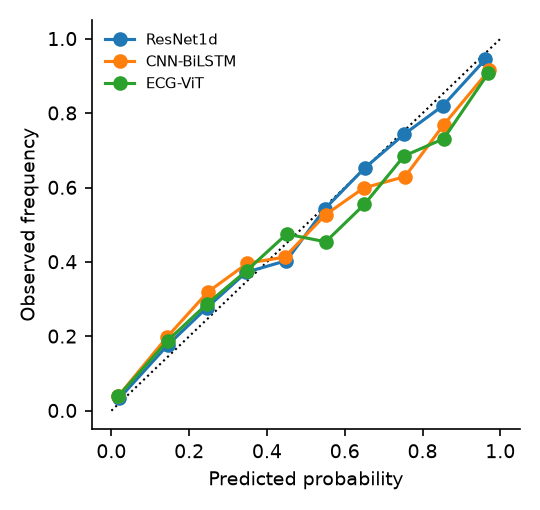
\includegraphics[width=0.45\linewidth]{fig6_reliability.png}
\caption{Reliability diagram of the 12-lead models (seed 0, all classes pooled).}
\end{figure}

\begin{figure}[H]
\centering
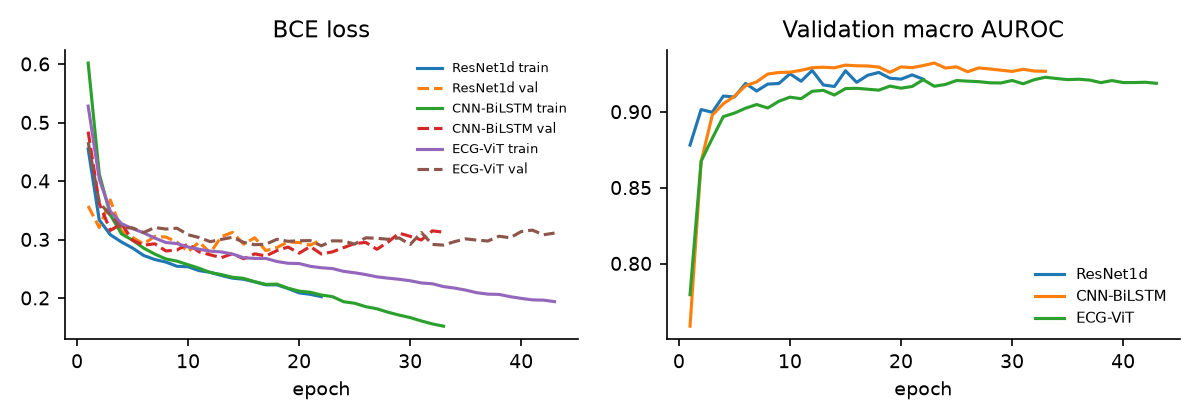
\includegraphics[width=0.85\linewidth]{fig7_training_curves.png}
\caption{Training and validation loss and validation macro AUROC of the 12-lead models (seed 0).}
\end{figure}

\begin{figure}[H]
\centering
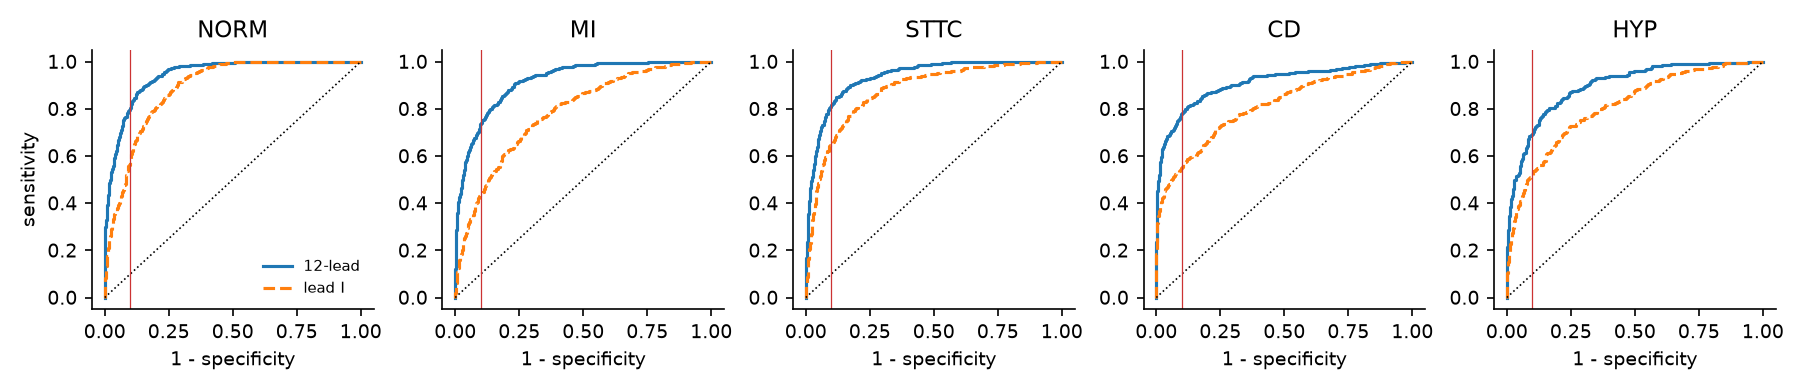
\includegraphics[width=\linewidth]{fig8_roc_12lead_vs_leadI.png}
\caption{Per-class ROC curves of ResNet1d with 12 leads and lead I (seed 0); the vertical line marks 90\% specificity.}
\end{figure}

\section{Reproducing the results}
\label{app:repro}
All code, launch scripts and result tables are in the submitted code archive. With the PTB-XL v1.0.3 data in \texttt{data/ptb-xl}, the full pipeline is:
\begin{enumerate}
  \item \texttt{python scripts/prepare\_data.py} -- build the 100\,Hz cache;
  \item \texttt{python scripts/baselines.py} -- E0 baselines B0--B2;
  \item \texttt{python scripts/run\_experiments.py --exp all} -- E1--E5 (102 runs; finished runs are skipped);
  \item \texttt{python scripts/e8\_self\_supervised.py} -- E8 pre-training and fine-tuning;
  \item \texttt{python scripts/external\_validation.py} \texttt{--data\_dir <WFDBRecords> --name chapman} -- E7;
  \item \texttt{python scripts/summarize.py}, \texttt{conclusion\_table.py}, \texttt{ensemble\_subgroup.py}, \texttt{explain.py} and \texttt{make\_paper\_figures.py} -- tables and figures.
\end{enumerate}
Exact commands, environment details and expected run times are given in the archive's \texttt{README.md}.


\end{document}
